\documentclass[a4paper]{article}
\usepackage{polski}
\usepackage[utf8]{inputenc}
\usepackage{enumerate}
\usepackage{graphicx}

\usepackage{geometry}
\newgeometry{tmargin=2.5cm, bmargin=2cm, lmargin=2cm, rmargin=2cm}

\title{Założenia projektowe, specyfikacja funkcjonalna, kryteria ewaluacji}
\date{}
\author{}

\begin{document}
\maketitle

\begin{enumerate}

\item Dekompozycja układu mechanicznego i elektronicznego:
%\begin{figure}
%\centering
%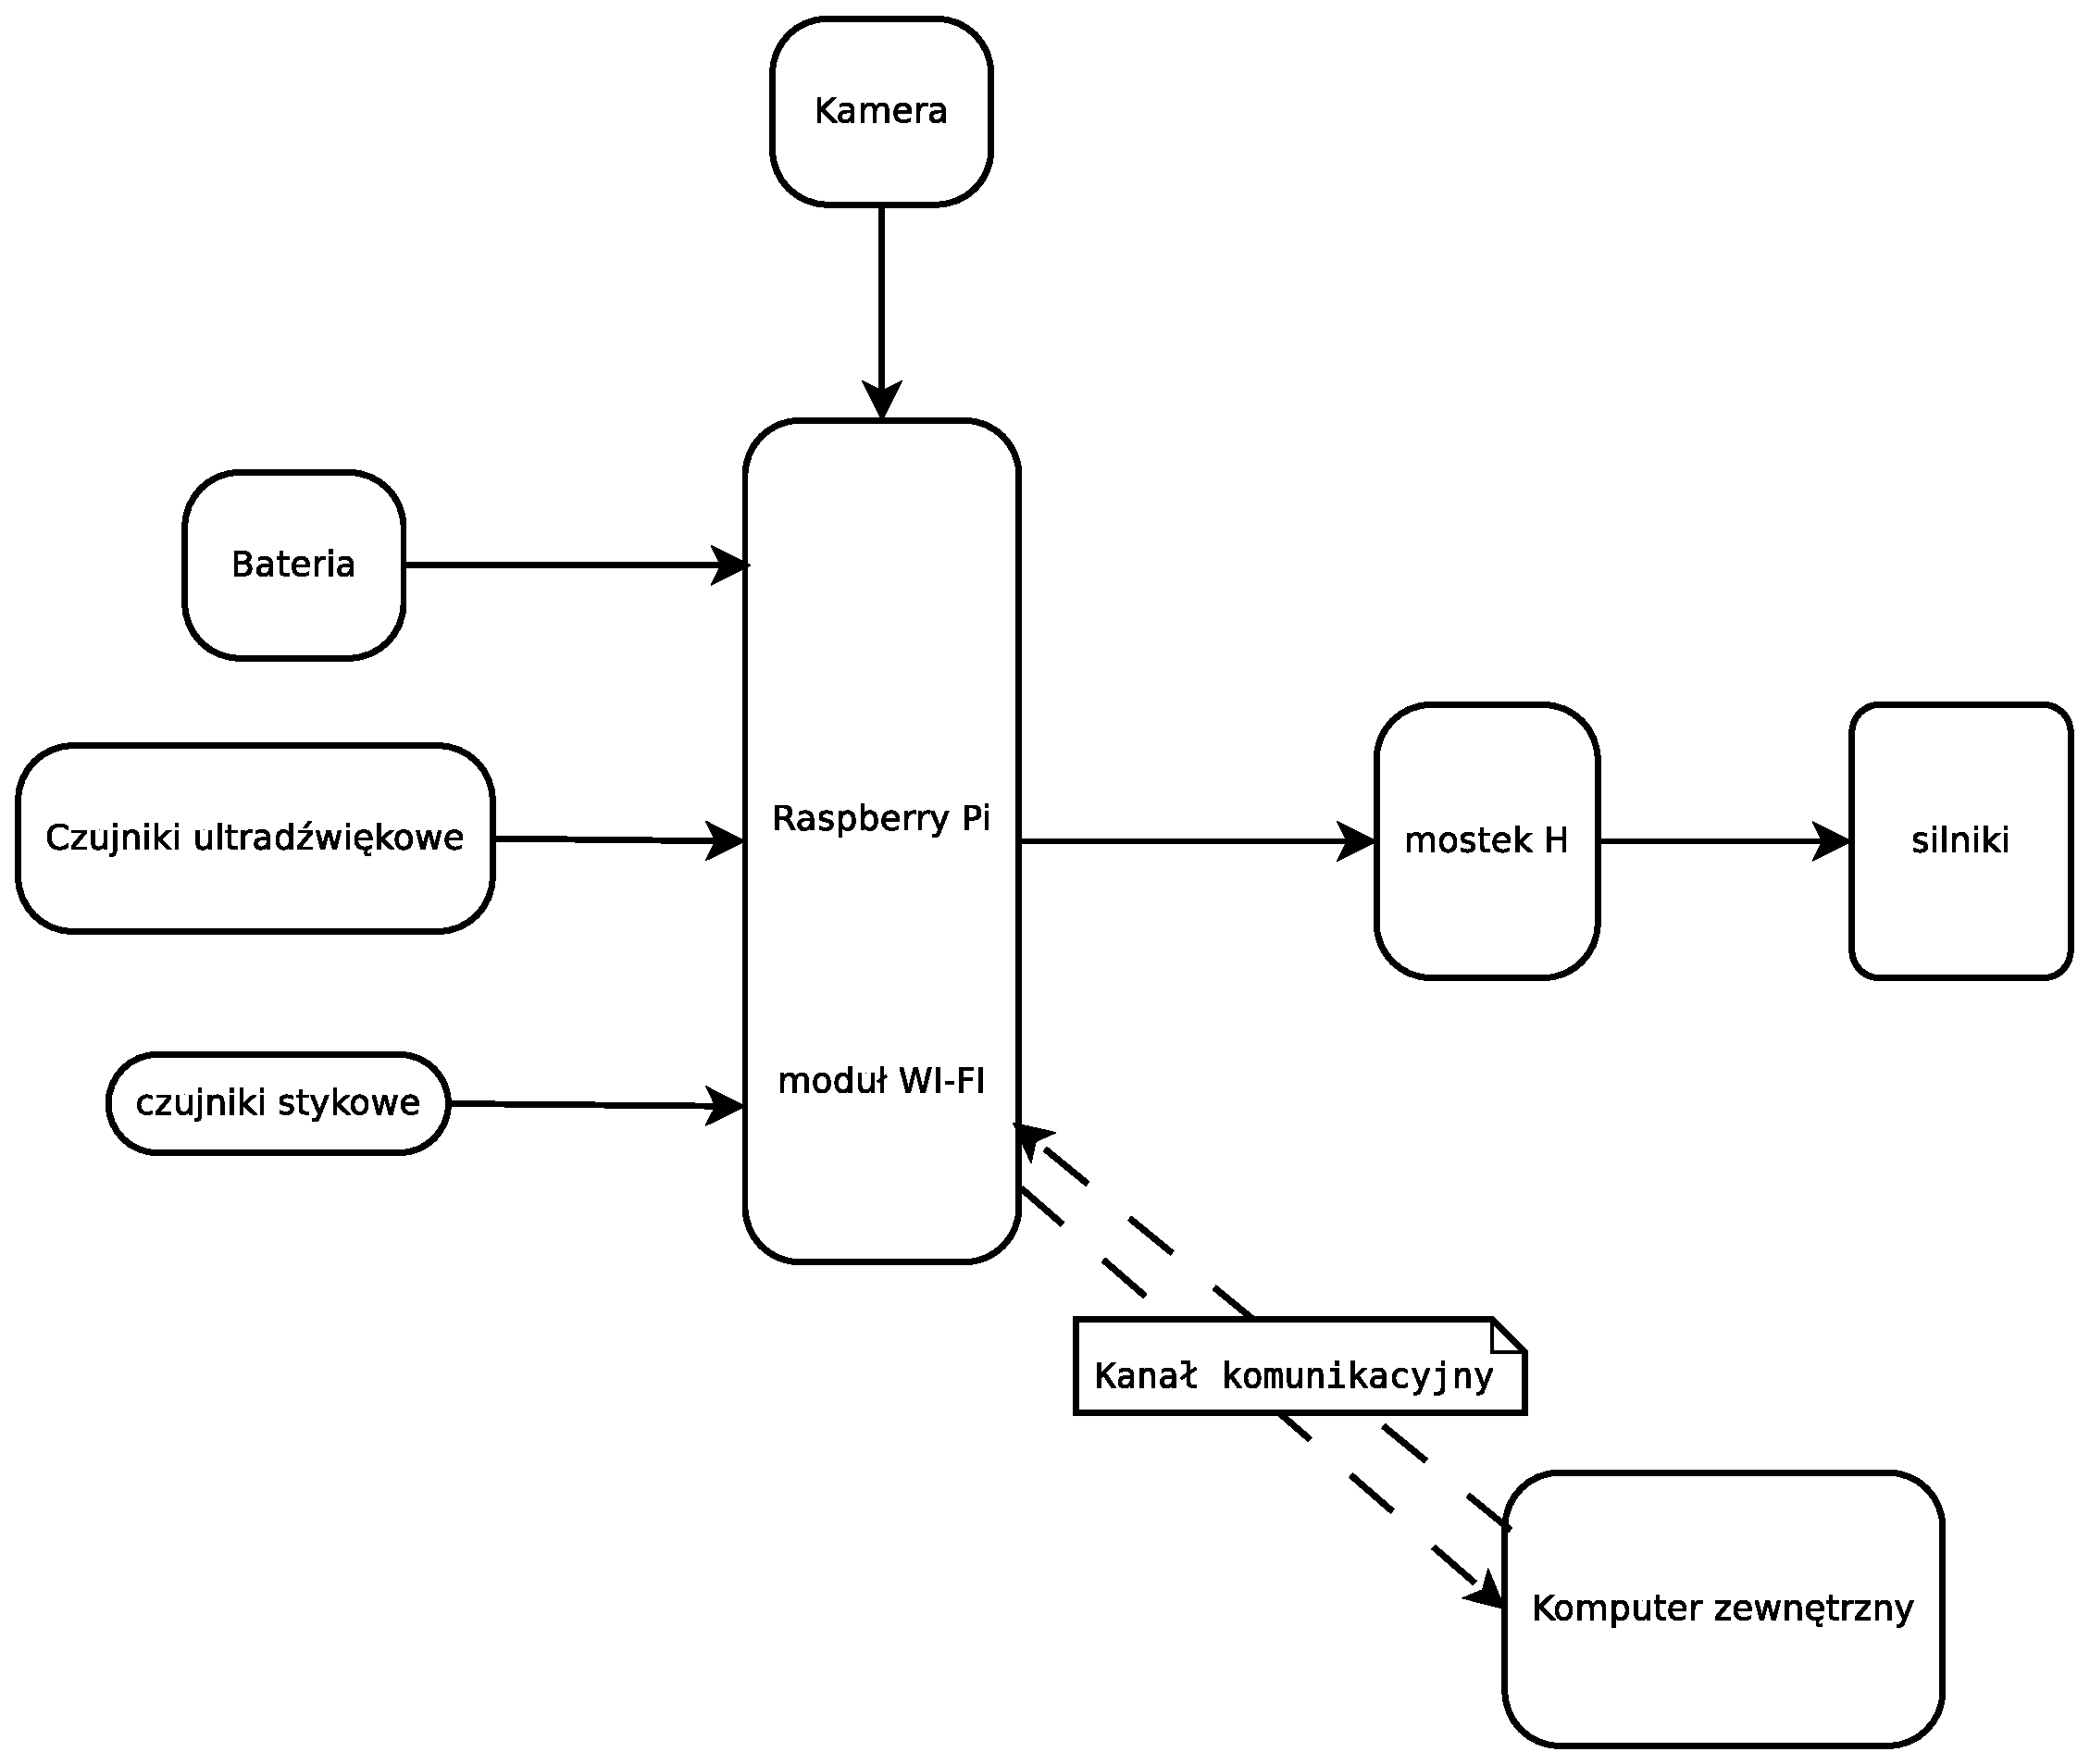
\includegraphics[scale=.7]{idea sprzet-mech.eps}
%\end{figure}

\item Dekompozycja oprogramowania:
%\begin{figure}
%\centering
%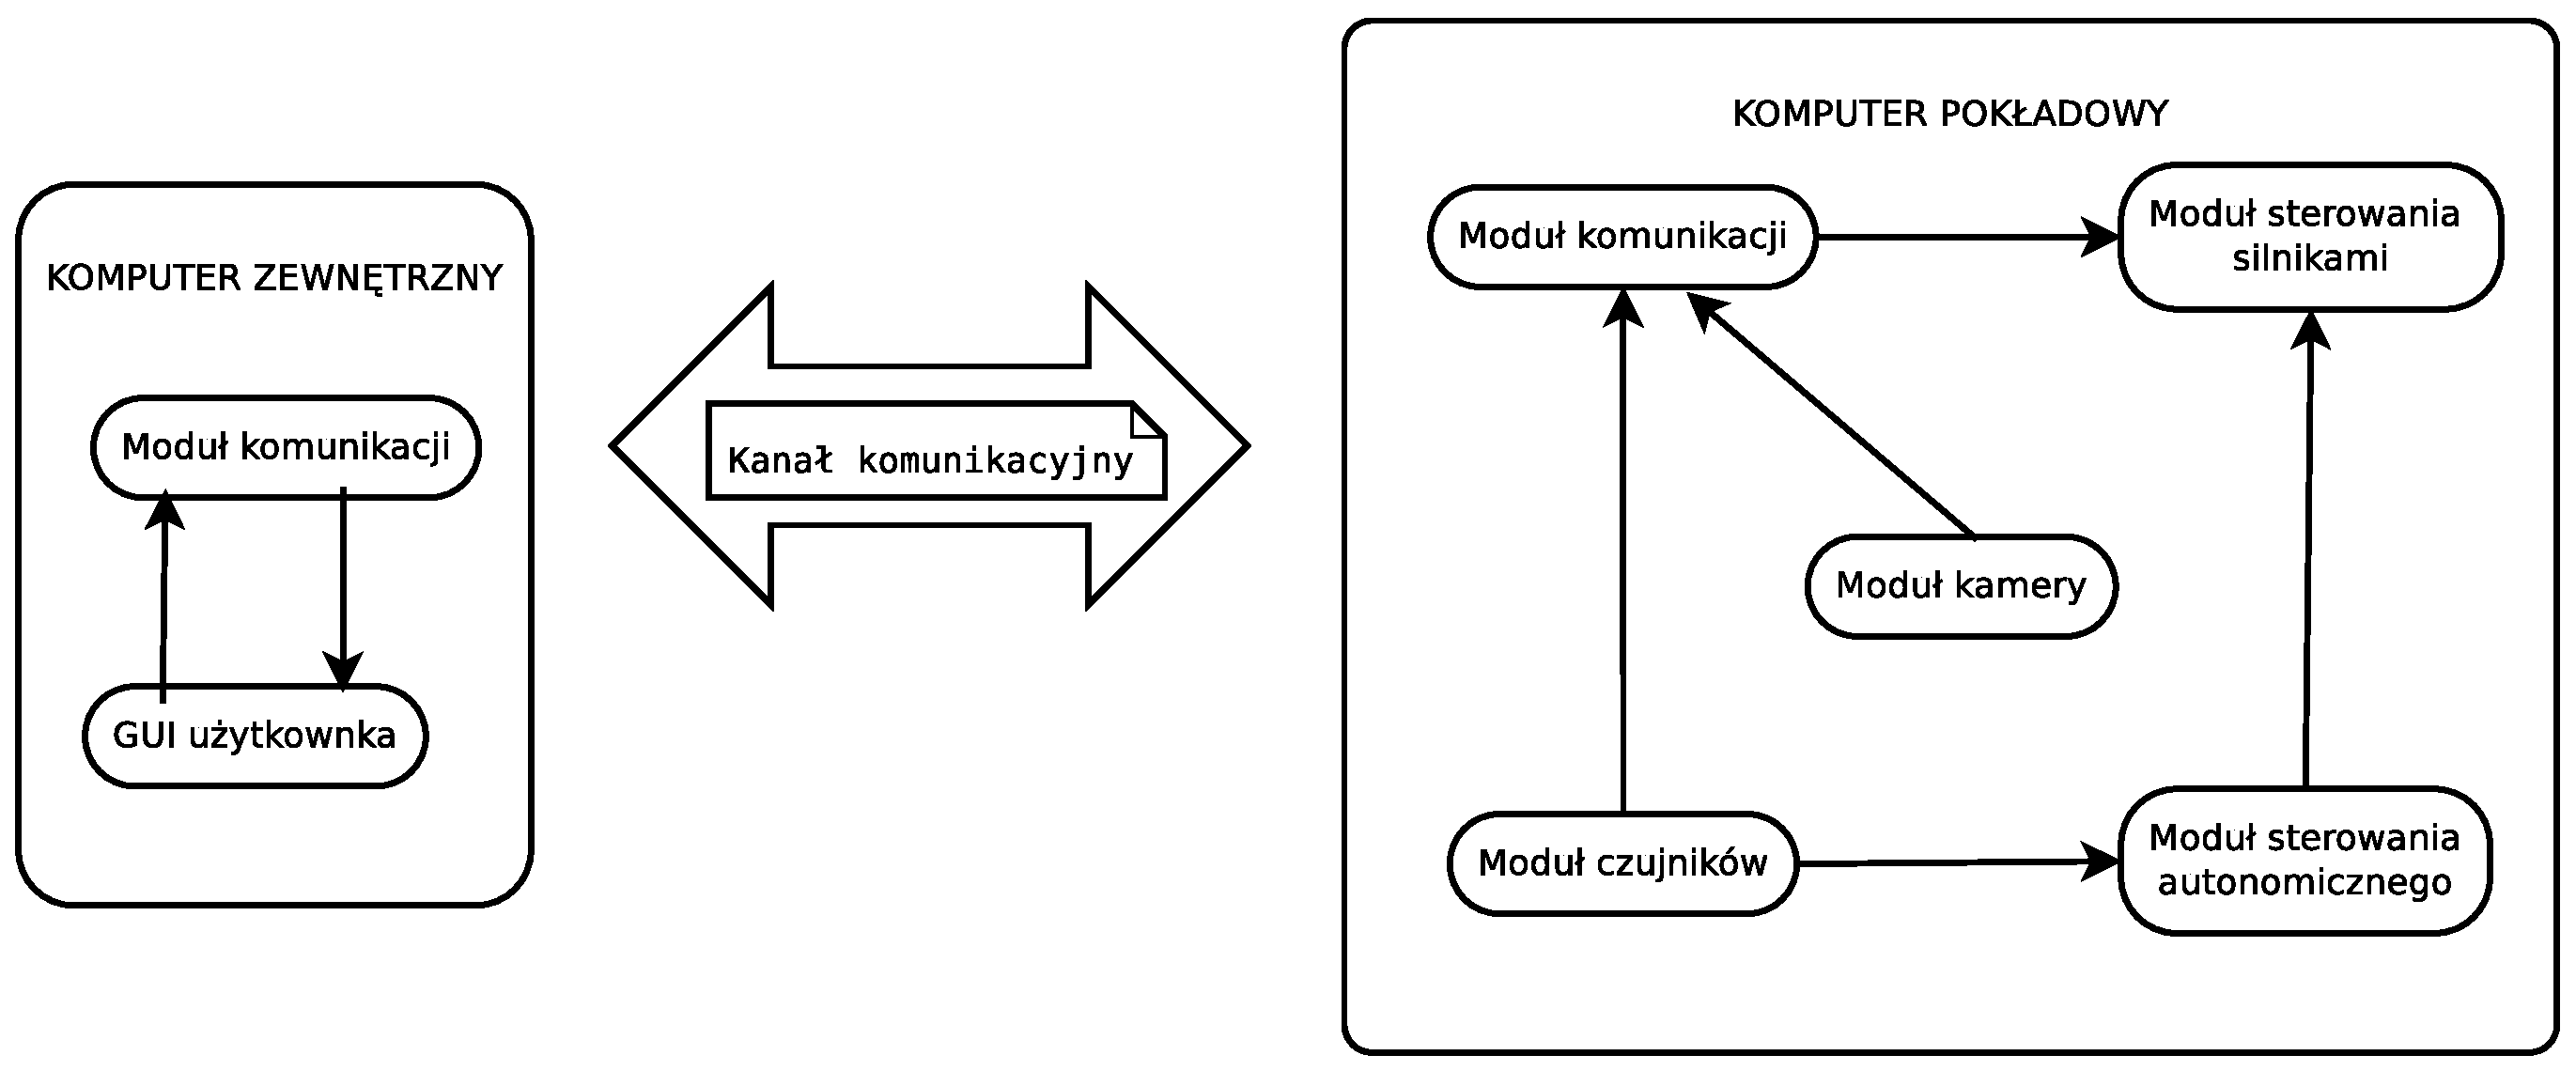
\includegraphics[scale=.7]{idea programowa.eps}
%\end{figure}

\item Opis komponentów:

\item Zależnosci we/wy:

\item Kryteria ewaluacji:

Robot czterokołowy umożliwi zdalne sterowanie w pomieszczeniu zamkniętym i dokonanie inspekcji pomieszczenia z zapisem video i sygnałów ze wszystkich czujników pomiarowych. Wykrywanie przeszkód odbywa się dwustopniowo: przez analizę danych z czujników ultradźwiękowych, oraz przez analizę danych odebranych z czujników stykowych. Po wykryciu przeszkody robot spróbuje ominąć przeszkodę. W razie braku możliwosci ominięcia przeszkody robot zatrzyma się.

\item Baza sprzętowa i programowa:

\end{enumerate}

\end{document}